\newpage
\begin{center}
  \textbf{\large 2 ТЕХНИЧЕСКАЯ РЕАЛИЗАЦИЯ}
\end{center}

\addcontentsline{toc}{section}{2 ТЕХНИЧЕСКАЯ РЕАЛИЗАЦИЯ}

\textbf{\large 2.1 Структура базы данных}
\addcontentsline{toc}{subsection}{2.1 Структура базы данных}

База данных для разрабатываемого приложения состоит из 4 таблиц (рис. 1). Ниже приведено описание каждой таблицы и связей между ними.

\renewcommand{\figurename}{Рисунок}
\begin{figure}[htbp]
    \centering % Центрируем изображение
    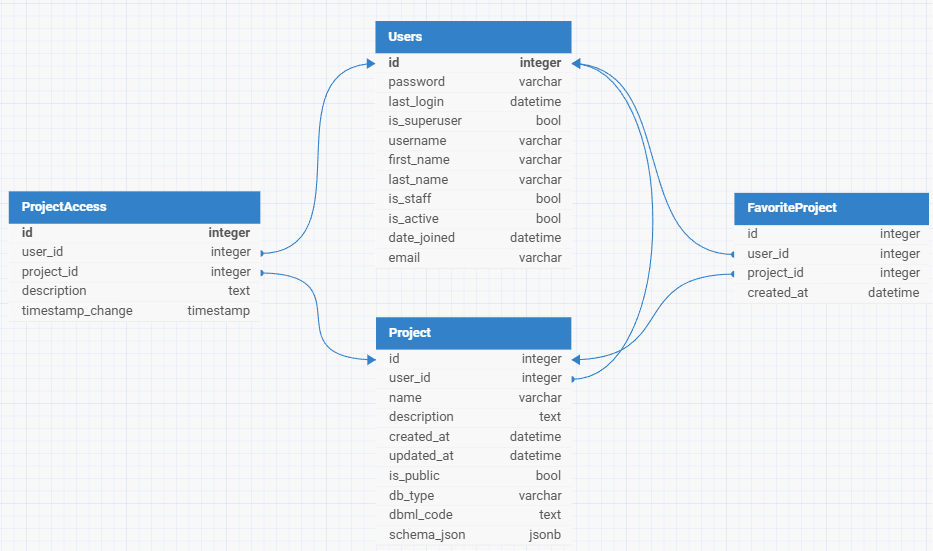
\includegraphics[width=1\textwidth]{db.png} 
    \caption{Структура базы данных}
    \label{fig:analyze} % Метка для ссылок
\end{figure}

Таблица User хранит информацию о зарегистрированных пользователях, их учетные данные и даты регистрации.

• id (integer, primary key, auto increment) – уникальный числовой идентификатор пользователя

• password (varchar(128) not null) – хешированное значение пароля для безопасной аутентификации

• last\_login (datetime null) – метка времени последнего успешного входа в систему

• is\_superuser (boolean not null) – флаг администраторских прав

• username (varchar(150) unique not null) – уникальное имя пользователя, обязательное поле

• first\_name (varchar(150) null) – имя пользователя

• last\_name (varchar(150) null) – фамилия пользователя

• email (varchar(254) unique not null) – электронная почта пользователя, используется для входа

• is\_staff (boolean not null) – флаг доступа к административной панели

• is\_active (boolean not null) – флаг активности учетной записи

• date\_joined (datetime not null) – дата и время регистрации пользователя


Таблица Project содержит данные о созданных пользователями проектах, представляющих собой схемы баз данных.

• id (integer, primary key, auto increment) – уникальный идентификатор проекта

• user\_id (integer not null) – ссылка на владельца проекта

• name (varchar(255) not null) – название проекта с ограничением длины

• description (text null) – описание проекта

• created\_at (datetime not null) – автоматически устанавливаемая дата 
создания

• updated\_at (datetime not null) – автоматически обновляемая дата изменения

• is\_public (boolean default true) – флаг публичной доступности проекта

• db\_type (varchar(20) not null) – тип СУБД (mysql/postgresql/sqlserver/Oracle)

• dbml\_code (text not null) – полное описание схемы в формате DBML

• schema\_json (jsonb not null) – структура проекта в JSON-формате

Таблица FavoriteProject (избранные проекты) - осуществляет связь между пользователями и добавленными в избранное проектами.

• id (integer, primary key, auto increment) – уникальный идентификатор записи

• user\_id (integer not null) – ссылка на пользователя

• project\_id (integer not null) – ссылка на проект

• created\_at (datetime not null) – дата добавления в избранное

Ограничения:
• Уникальный составной индекс (user\_id, project\_id) предотвращает дублирование

• Каскадное удаление при удалении связанных записей

Таблица ProjectAccess (права доступа) - управляет разрешениями пользователей для работы с проектами.

• id (integer, primary key, auto increment) – уникальный идентификатор доступа

• project\_id (integer not null) – ссылка на проект

• user\_id (integer not null) – ссылка на пользователя

• role (varchar(10) not null) – уровень доступа (owner/editor/viewer)

• created\_at (datetime not null) – дата предоставления доступа

Роли доступа:

• owner – полные права владельца

• editor – права на редактирование

• viewer – права только на просмотр

Ограничения:

• Уникальный составной индекс (project\_id, user\_id) для исключения дублирования прав

• Каскадное удаление связанных записей

Связи между таблицами

1. User - Project (один-ко-многим):
Один пользователь (CustomUser) может быть владельцем множества проектов (Project). Связь реализована через поле user\_id в таблице Project, которое ссылается на id в CustomUser. При удалении пользователя все его проекты также удаляются (каскадное удаление).

2. User - FavoriteProject - Project (многие-ко-многим):
Пользователи могут добавлять проекты в избранное. Связь организована через промежуточную таблицу FavoriteProject, где user\_id ссылается на CustomUser, а project\_id - на Project. Уникальный индекс на пару этих полей предотвращает дублирование.

3. User - ProjectAccess - Project (многие-ко-многим):
Система управления доступом к проектам. Таблица ProjectAccess связывает пользователей с проектами через поля user\_id и project\_id, с указанием роли доступа (owner/editor/viewer). Уникальный индекс гарантирует, что каждый пользователь имеет только одну роль в конкретном проекте.

Все связи реализованы с каскадным удалением: при удалении пользователя или проекта автоматически удаляются связанные записи в FavoriteProject и ProjectAccess.


Предложенная структура обеспечивает удобную работу с проектами по моделированию баз данных, включая создание таблиц, полей и связей между ними. 

\

\textbf{\large 2.1.1 Нормализация базы данных}
\addcontentsline{tocdepth}{subsubsection}{2.1.1 Нормализация базы данных}

Таблица User (Пользователи) соответствует третьей нормальной форме (3NF). Первичный ключ id уникально идентифицирует каждого пользователя.
Все атрибуты полностью функционально зависят от первичного ключа. 
Отсутствуют транзитивные зависимости между неключевыми атрибутами. Структура таблицы не содержит повторяющихся групп данных, что соответствует требованиям первой нормальной формы (1NF). Нет частичных зависимостей неключевых атрибутов от первичного ключа, что удовлетворяет второй нормальной форме (2NF).

Таблица Project (Проекты) соответствует третьей нормальной форме. Первичный ключ id однозначно идентифицирует каждый проект. Все атрибуты зависят только от первичного ключа. 
Внешний ключ user\_id корректно связывает проект с владельцем из таблицы CustomUser. Поле schema\_json (тип JSONB) рассматривается как атомарное значение в контексте нормализации. Отсутствуют повторяющиеся группы данных и транзитивные зависимости.

Таблица FavoriteProject (Избранные проекты) соответствует третьей нормальной форме. Составной первичный ключ уникально идентифицирует каждую запись об избранном проекте. Поле created\_at полностью зависит от составного ключа. Внешние ключи user\_id и project\_id поддерживают целостность связей с соответствующими таблицами. Уникальный индекс на пару (user\_id, project\_id) предотвращает дублирование записей. Структура таблицы не содержит избыточных данных или транзитивных зависимостей.

Таблица ProjectAccess (Права доступа) соответствует третьей нормальной форме. Составной первичный ключ (project\_id, user\_id) уникально идентифицирует каждое право доступа. Поля role и created\_at полностью зависят от составного ключа. Внешние ключи project\_id и user\_id обеспечивают ссылочную целостность с таблицами Project и CustomUser соответственно. Система ролей (owner/editor/viewer) реализована без избыточности данных. Отсутствуют транзитивные зависимости между атрибутами.

Все связи между таблицами организованы в соответствии с принципами реляционной модели данных:

1. Связь «один-ко-многим» между CustomUser и Project реализована через внешний ключ user\_id в таблице Project с каскадным удалением, что обеспечивает целостность данных при удалении пользователя.

2. Связь «многие-ко-многим» между пользователями и избранными проектами реализована через промежуточную таблицу FavoriteProject с составным первичным ключом и соответствующими внешними ключами.

3. Связь «многие-ко-многим» между пользователями и проектами с разными уровнями доступа реализована через таблицу ProjectAccess с контролем уникальности сочетания project\_id и user\_id.

Все внешние ключи настроены на каскадное удаление, что поддерживает целостность данных при удалении родительских записей. Отсутствуют циклические зависимости и нарушения реляционных принципов.

\

\textbf{\large 2.2 Алгоритм синхронизации DBML и диаграммы}
\addcontentsline{toc}{subsection}{2.2 Алгоритм синхронизации DBML и диаграммы}

Система поддерживает двустороннюю синхронизацию между DBML-представлением и визуальной диаграммой. Это позволяет пользователям редактировать структуру базы данных как в текстовом формате DBML, так и через визуальный интерфейс, при этом изменения автоматически синхронизируются между обоими представлениями.

\textbf{\large 2.2.1 Структуры данных}
\addcontentsline{tocdepth}{subsubsection}{2.3.1 Структуры данных}

DBML-представление хранится в виде текстового формата (Листинг 1).

Листинг 1 - Структура DBML кода.
\begin{lstlisting}[frame=single]
    Table table_name {
      field_name field_type [constraints]
      ...
    }
    Ref: table1.field > table2.field
\end{lstlisting}

Диаграммное представление структуры базы данных (Листинг 2) храниться в виде словаря, состоящего из узлов, которые представляют каждую таблицу  и содержат следующие обязательные атрибуты:

• key (String) - уникальное название таблицы;

• location (Point) - координаты расположения узла на холсте в пикселях (x, y);

• items (массив) - поля таблицы. Каждое поле содержит в себе id (уникальный идентификатор поля в пределах таблицы), name (название поля), type (тип данных поля), isKey (флаг первичного ключа). 

Каждая связь между узлами описывает отношение между таблицами и содержит в себе информацию о таблицах, между которыми связь, информацию о портах, к которым будет присоединена стрелка связи и категорию, то есть тип связи (Листинг 2). 

Листинг 2 - Структура данных диаграммы.
\begin{lstlisting}[frame=single]
const nodeDataArray = [
    {
        key: "User",
        location: new go.Point(200, 0),
        items: [
            {
                id: 1, name: "id", iskey: true,
                type: "integer"
            },
            { id: 2, name: "name", type: "varchar(255)" }
        ]
    },
    {
        key: 'Project',
        location: new go.Point(500, 0),
        items: [
            {
                id: 1, name: 'id', iskey: true,
                type: "integer"
            },
            { id: 2, name: 'name', type: "varchar(255)" },
        ]
    }
];

const linkDataArray = [
    {
        from: 'User',
        to: 'Project',
        fromPort: 'right_1',
        toPort: 'left_1',
        category: "many-to-one"
    },
];
\end{lstlisting}


\textbf{\large 2.2.2 Преобразование DBML в диаграмму}
\addcontentsline{tocdepth}{subsubsection}{2.2.2 Преобразование DBML в диаграмму}

Процесс преобразования текстового DBML-описания в интерактивную диаграмму начинается с парсинга исходного текста (Листинг 3). Сначала система анализирует текст, выделяя декларации таблиц и отношений между ними. Для каждой найденной таблицы создается соответствующий узел диаграммы. Узел содержит название таблицы и список ее полей, где каждое поле получает уникальный идентификатор, используемый в дальнейшем для установки связей. Поля, помеченные как первичные ключи, получают специальный флаг iskey.

После создания всех узлов система обрабатывает объявления отношений (Ref). Для каждого отношения определяется исходная и целевая таблицы, а также конкретные поля, участвующие в связи. На диаграмме это отображается в виде соединения между соответствующими портами узлов-таблиц. Левые порты используются для входящих связей, правые — для исходящих. Тип связи (один-к-одному, один-ко-многим или многие-к-одному) определяется на основе анализа DBML-описания и влияет на визуальное отображение стрелки связи.

Листинг 3 - Функция преобразования DBML в диаграмму.
\begin{lstlisting}[frame=single]
 const lines = dbml.split('\n');
    lines.forEach(line => {
        line = line.trim();

        if (line.startsWith('Table')) {
            if (currentTable) {
                tables.set(currentTable, currentItems);
                const existingPos = existingPositions
                    .get(currentTable);
                const position = existingPos ?
                    new go.Point(existingPos.x, 
                        existingPos.y):
                    new go.Point(currentX, currentY);

                model.addNodeData({
                    key: currentTable,
                    items: currentItems,
                    location: position
                });

                if (!existingPos) {
                    currentX += spacing;
                    if (currentX > 900) {
                        currentX = 0;
                        currentY += spacing;
                    }
                }
            }
            const match = line.match(/Table\s+(\w+)/);
            if (match) {
                currentTable = match[1];
                currentItems = [];
            }
        }
        else if (line && !line.startsWith('Ref:') 
                && !line.startsWith('}')) {
            const fieldMatch = line.match(/(\w+)\s+(\w+)/);
            if (fieldMatch) {
                const [_, name, type] = fieldMatch;
                const isKey = line.includes('[primary key]');
                const fieldId = Date.now() + Math.random();
                currentItems.push({
                    id: fieldId,
                    name: name,
                    type: type,
                    iskey: isKey
                });
            }
        }
    });
\end{lstlisting}

\textbf{\large 2.2.3 Преобразование диаграммы в DBML}
\addcontentsline{tocdepth}{subsubsection}{2.2.3 Преобразование диаграммы в DBML}

Обратный процесс преобразования текущего состояния диаграммы в DBML формат начинается с обхода всех узлов-таблиц (Листинг 4). Для каждой таблицы формируется соответствующая секция Table в DBML, включающая все ее поля с указанием типов данных и отметками о первичных ключах. Поля сохраняют свои исходные имена из диаграммы, а их уникальные идентификаторы используются только для внутреннего сопоставления.

Далее система анализирует все связи между таблицами. Для каждой связи определяется, какие конкретно поля таблиц соединены (через анализ portId), и формируется соответствующая строка Ref в DBML. Направление связи соответствует направлению внешнего ключа в реляционной модели. Тип связи в текущей реализации не отражается в DBML-коде, так как стандарт DBML не предусматривает явного указания этого параметра.

Листинг 4 - Функция преобразования диаграммы в DBML.
\begin{lstlisting}[frame=single]
function diagramToDBML() {
    let dbml = '';
    const nodes = myDiagram.nodes;
    const links = myDiagram.links;

    nodes.each(node => {
        if (!node || !node.data || !node.data.key) return;
        const tableName = node.data.key;
        dbml += `Table ${tableName} {\n`;

        if (node.data.items
                && Array.isArray(node.data.items)) {
            node.data.items.forEach(item => {
                if (!item || !item.name || !item.type) 
                return;

                let field = `  ${item.name} ${item.type}`;
                if (item.iskey) {
                    field += ' [primary key]';
                }
                dbml += field + '\n';
            });
        }
        dbml += '}\n\n';
    });

    links.each(link => {
        if (!link) return;

        const fromNode = link.fromNode;
        const toNode = link.toNode;
        if (!fromNode || !toNode 
            || !fromNode.data || !toNode.data) return;

        const fromPort = link.fromPort;
        const toPort = link.toPort;
        if (!fromPort || !toPort 
            || !fromPort.portId || !toPort.portId) return;

        const fromFieldId = fromPort.portId.split('_')[1];
        const toFieldId = toPort.portId.split('_')[1];

        const fromField = fromNode.data.items.find(
            item => String(item.id) === String(fromFieldId)
        );
        const toField = toNode.data.items.find(
            item => String(item.id) === String(toFieldId)
        );

        if (fromField && toField) {
            dbml += `Ref: ${fromNode.data.key}.
            ${fromField.name} > ${toNode.data.key}
            .${toField.name}\n`;
        }
    });

    return dbml;
}
\end{lstlisting}

\textbf{\large 2.2.4 Механизм синхронизации DBML и диаграммы}
\addcontentsline{tocdepth}{subsubsection}{2.2.4 Механизм синхронизации DBML и диаграммы}

Синхронизация между текстовым редактором и диаграммой реализована через систему взаимных подписок на изменения. При любом изменении в диаграмме (добавление/удаление элементов, изменение свойств) срабатывает обработчик, который через небольшой промежуток времени (100мс) генерирует актуальный DBML и обновляет содержимое текстового редактора. Аналогично, при изменениях в текстовом редакторе система парсит новый DBML и соответствующим образом обновляет диаграмму (Листинг 5).

Листинг 5 - Обработчик изменения диаграммы.
\begin{lstlisting}[frame=single]
    myDiagram.addDiagramListener("ChangedSelection",
        function (e) {
            if (isUpdatingFromDiagram) return;
            const dbml = diagramToDBML();
            if (window.editor
                && window.editor.getValue() !== dbml) {
                isUpdatingFromDiagram = true;
                window.updateEditorFromDiagram(dbml);
                setTimeout(() => {
                    isUpdatingFromDiagram = false;
                }, 100);
            }
        });
\end{lstlisting}

Для предотвращения бесконечных циклов обновления используется флаг isUpdating, который временно блокирует обработчики изменений при выполнении синхронизации в одном из направлений. Это гарантирует, что каждое изменение будет обработано только один раз, и система быстро придет к согласованному состоянию (Листинг 6).

Листинг 6 - Функция debounce.
\begin{lstlisting}[frame=single]
let isUpdatingFromDiagram = false;

function debounce(func, wait) {
    let timeout;
    return function executedFunction(...args) {
        const later = () => {
            clearTimeout(timeout);
            func(...args);
        };
        clearTimeout(timeout);
        timeout = setTimeout(later, wait);
    };
}
\end{lstlisting}

На Рисунке 2 представлена BPMN диаграмма процесса выгрузки SQL-дампа.

\renewcommand{\figurename}{Рисунок}
\begin{figure}[htbp]
    \centering % Центрируем изображение
    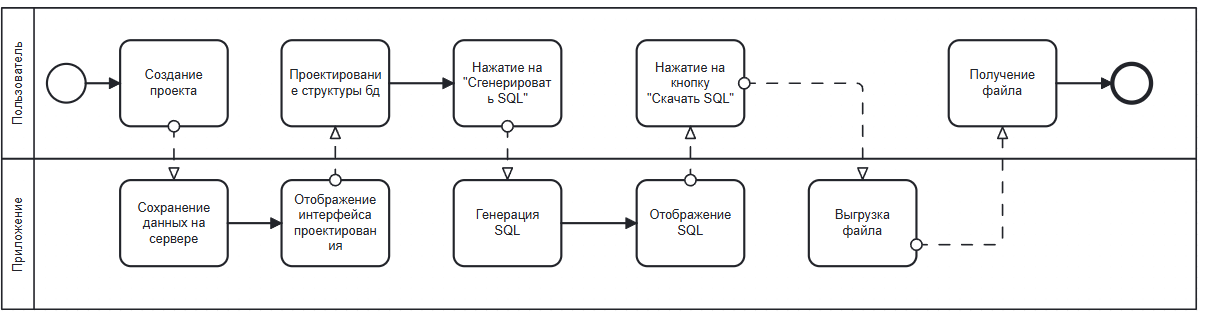
\includegraphics[width=1\textwidth]{bpmn.png} 
    \caption{BPMN диаграмма процесса выгрузки SQL}
    \label{fig:analyze} % Метка для ссылок
\end{figure}

\newpage
\textbf{\large 2.3 Алгоритм преобразования DBML в SQL}
\addcontentsline{toc}{subsection}{2.3 Алгоритм преобразования DBML в SQL}

Система предоставляет возможность конвертации DBML-схемы в SQL-скрипт для создания базы данных. Процесс конвертации происходит через цепочку взаимодействий между фронтендом, бэкендом и Node.js-скриптом конвертации.

На Рисунке 3 представлена UML диаграмма процесса выгрузки SQL-дампа из приложения. Пользователю представлен выбор метода проектирования базы данных: с помощью графического интерфейса или посредством DBML.

\renewcommand{\figurename}{Рисунок}
\begin{figure}[htbp]
    \centering % Центрируем изображение
    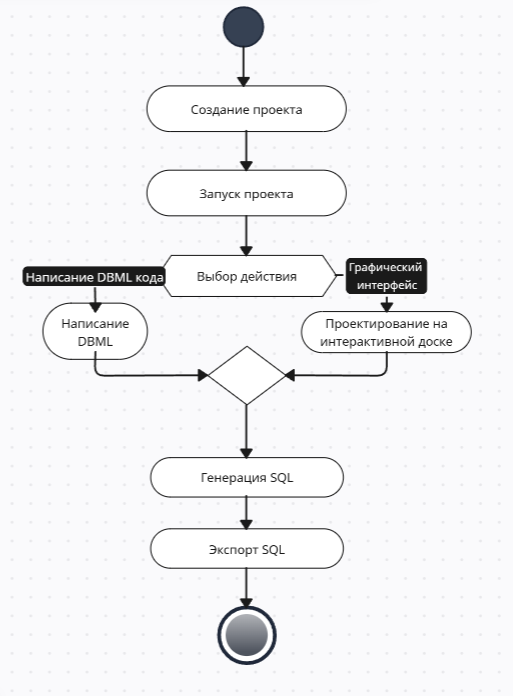
\includegraphics[height=0.6\textwidth]{uml.png} 
    \caption{UML диаграмма процесса выгрузки SQL}
    \label{fig:analyze} % Метка для ссылок
\end{figure}

Процесс начинается на фронтенде, когда пользователь нажимает кнопку экспорта SQL. Обработчик события для кнопки exportSqlBtn получает текущий DBML-код из редактора Monaco, затем отправляет POST-запрос на адрес /builder/convert-dbml/. В теле запроса передается dbml-код и тип базы данных, ранее выбранный пользователем, для которого нужно будет сгенерировать SQL (Листинг 7).

\newpage
Листинг 7 - Обработчик события для кнопки exportSqlBtn.
\begin{lstlisting}[frame=single]
document.getElementById('exportSqlBtn')
    .addEventListener('click',
        async function () {
            const dbmlCode = editor.getValue();
            try {
                const response = await fetch(
                '/builder/convert-dbml/', {
                    method: 'POST',
                    headers: {
                        'Content-Type': 'application/json',
                        'X-CSRFToken': getCookie('csrftoken')
                    },
                    body: JSON.stringify({
                        dbml: dbmlCode,
                        db_type: window.DB_TYPE
                    })
                });

                if (!response.ok) {
                    throw new Error(await response.text());
                }

                const sqlCode = await response.text();

                const blob = new Blob([sqlCode], 
                        { type: 'text/sql' });
                const url = URL.createObjectURL(blob);
                const a = document.createElement('a');
                a.href = url;
                a.download = 'database_dump.sql';
                document.body.appendChild(a);
                a.click();
                document.body.removeChild(a);
                URL.revokeObjectURL(url);

            } catch (error) {
                console.error('Export failed:', error);
            }
        });
\end{lstlisting}

На серверной стороне определен обработчик conver\_dbml\_to\_sql (Листинг 8), который принимает POST-запрос с JSON-данными и извлекает DBML-код и тип базы данных. Затем запускается Node.js-скрипт convert.js через subprocess (библиотека Python). Данные в скрипте передаются через stdin, результат конвертации принимается через stdout.

Листинг 8 - Функция convert\_dbml\_to\_sql.
\begin{lstlisting}[frame=single]
@csrf_exempt
def convert_dbml_to_sql(request):
    if request.method == 'POST':
        if request.content_type == 'application/json':
            data = json.loads(request.body)
            dbml_code = data.get('dbml')
            db_type = data.get('db_type', 'mysql')
        else:
            dbml_code = request.body.decode('utf-8')
            db_type = 'mysql'

        process = subprocess.Popen(
            ['node', 'convert.js'],
            stdin=subprocess.PIPE,
            stdout=subprocess.PIPE,
            stderr=subprocess.PIPE
        )
        input_data = json.dumps({
            'dbml': dbml_code,
            'db_type': db_type
        })

        stdout, stderr = process.communicate(
            input=input_data.encode('utf-8')
        )
        if process.returncode != 0:
            return HttpResponse(f'Error: 
            {stderr.decode("utf-8")}', status=500)
        return HttpResponse(stdout, 
            content_type='text/plain')
    return HttpResponse('Only POST method is allowed', 
            status=405)
\end{lstlisting}

Скрипт convert.js использует библиотеку @dbml/core для конвертации 
DBML в SQL. Скрипт получает входные данные и парсит JSON с DBML-кодом и выбранным типом базы данных. Перед парсингом проверяет поддержку типа базы данных. После выводит результат в stdout, который далее получает функция convert\_dbml\_to\_sql (Листинг 8). После успешной конвертации проверяется код возврата процесса. В случае ошибки возвращается сообщение об ошибке, а при успехе возвращается сгенерированный SQL-код. Далее обработчик события кнопки exportSqlBtn (Листинг 7) создается Blob с SQL-кодом и генерирует временную ссылку для скачивания. После завершения процесса скачиваения очищаются временные ресурсы.


\newpage
\textbf{\large 2.4 Проектирование интерфейса}
\addcontentsline{toc}{subsection}{2.4 Проектирование интерфейса}

В интерфейсе приложения используются цвета, которые обеспечивают
хорошую читаемость и визуальный комфорт. Основные цвета, выбранные для
оформления интерфейса:
- фоновый цвет: светло-серый или белый (#f5f5f5 или #ffffff) —
используется для основного фона окон и панелей;
- цвет панелей и карточек: белый (#ffffff) с лёгкой тенью или рамкой для
отделения элементов друг от друга;
- цвет шапки сайта: серый (#343a40).
- основной акцентный цвет: насыщенный синий (#1976d2) —
применяется для кнопок, выделения активных элементов, ссылок и
заголовков;
- цвет кнопки выхода: ярко-желтый (#ffc107) с эффектом наведения
(светло-желтый #ffca2c);
- цвет кнопки «Новый проект»: синийй (#ffd600);
- цвет текста: тёмно-серый или белый (#222222 или #ffffff);
- цвет рамок и разделителей: светло-серый (#e0e0e0 или #cccccc).
Также используются плавные эффекты наведения (hover) для кнопок и
интерактивных элементов, чтобы интерфейс выглядел современно и
отзывчив.

\textbf{\large 2.4.1 Страница авторизации}
\addcontentsline{tocdepth}{subsubsection}{2.5.1 Страница авторизации}

На данную страницу можно перейти после нажатия на кнопку "Войти". В
центре окна расположены поля для ввода email и пароля. При ошибках (например,если поля не заполнены или введены неверные данные) появляются
всплывающие сообщения. Все элементы аккуратно выровнены и оформлены
в едином стиле (Рисунок 4).

\renewcommand{\figurename}{Рисунок}
\begin{figure}[htbp]
    \centering % Центрируем изображение
    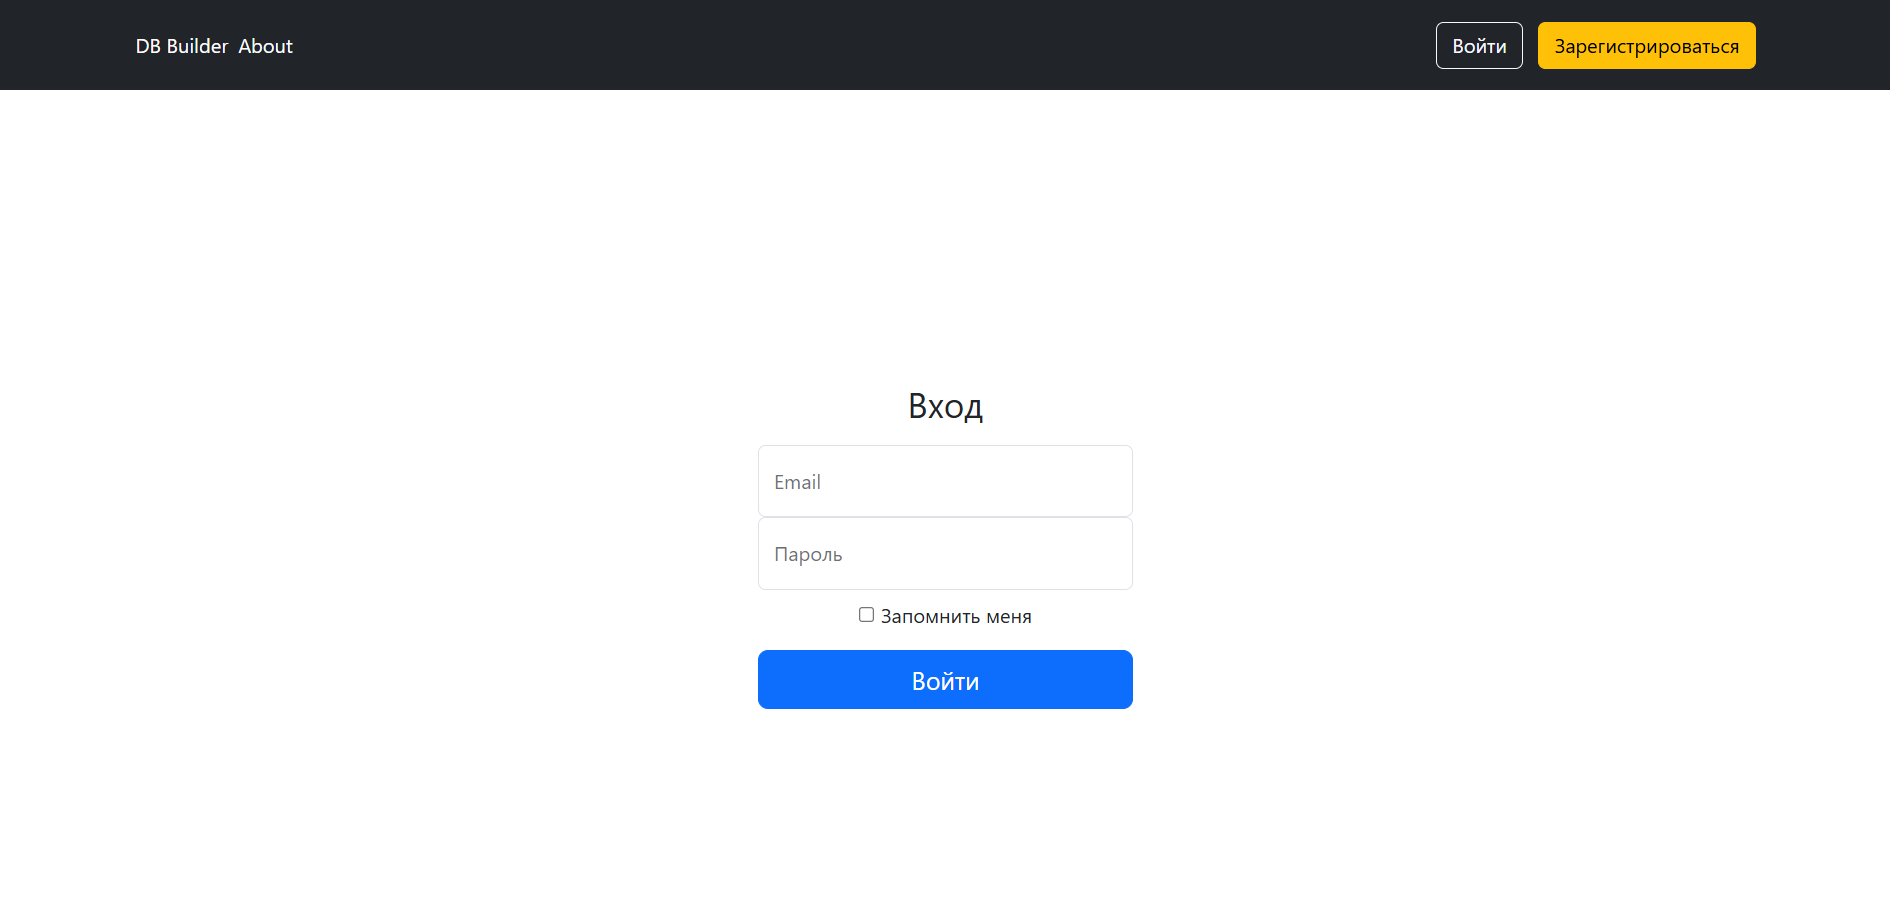
\includegraphics[height=0.45\textwidth]{img/auth.png}
    \caption{Cтраница авторизации}
    \label{fig:analyze} % Метка для ссылок
\end{figure}

\textbf{\large 2.4.2 Страница регистрации}
\addcontentsline{tocdepth}{subsubsection}{2.5.2 Страница регистрации}

На данную страницу можно перейти после нажатия на кнопку "Зарегистрироваться". Здесь пользователь вводит логин, email, пароль и подтверждение пароля. Есть кнопка возврата к окну авторизации. Если логин уже занят, пароли не совпадают или не заполнены обязательные поля, пользователю выводится соответствующее сообщение об ошибке. Окно выполнено в том же стиле, что и авторизация, с понятными подписями и подсказками в полях ввода (Рисунок 5).

\newpage
\renewcommand{\figurename}{Рисунок}
\begin{figure}[htbp]
    \centering % Центрируем изображение
    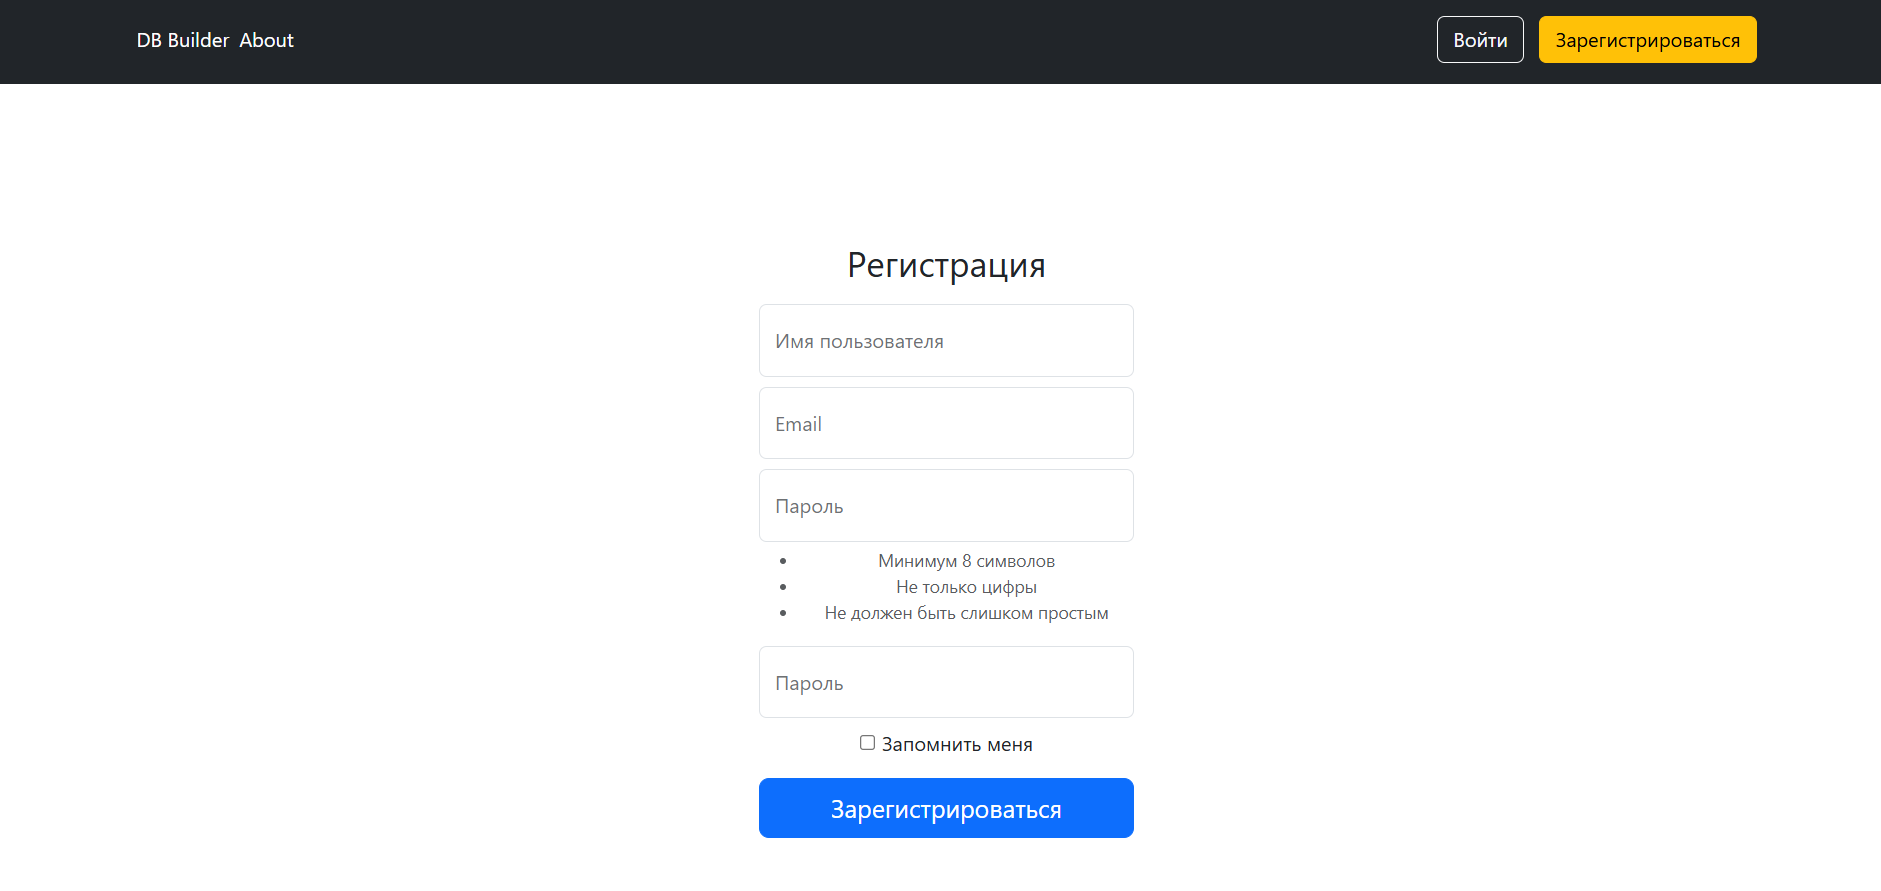
\includegraphics[height=0.45\textwidth]{img/signup.png}
    \caption{Cтраница регистрации}
    \label{fig:analyze} % Метка для ссылок
\end{figure}


\textbf{\large 2.4.3 Домашняя страница}
\addcontentsline{tocdepth}{subsubsection}{2.4.3 Домашняя страница}

Это главная страница веб-приложения, на которой содержится описание проекта.
В шапке страницы есть кнопки для входа и регистрации или кнопка выхода, если пользователь уже авторизован. В основном блоке содержится информация о проекте, а также кнопка "Попробовать редактор" , при клике на которую пользователь попадает либо на страницу авторизации, если он не авторизован, либо на страницу проектов (Рисунок 6).

\renewcommand{\figurename}{Рисунок}
\begin{figure}[htbp]
    \centering % Центрируем изображение
    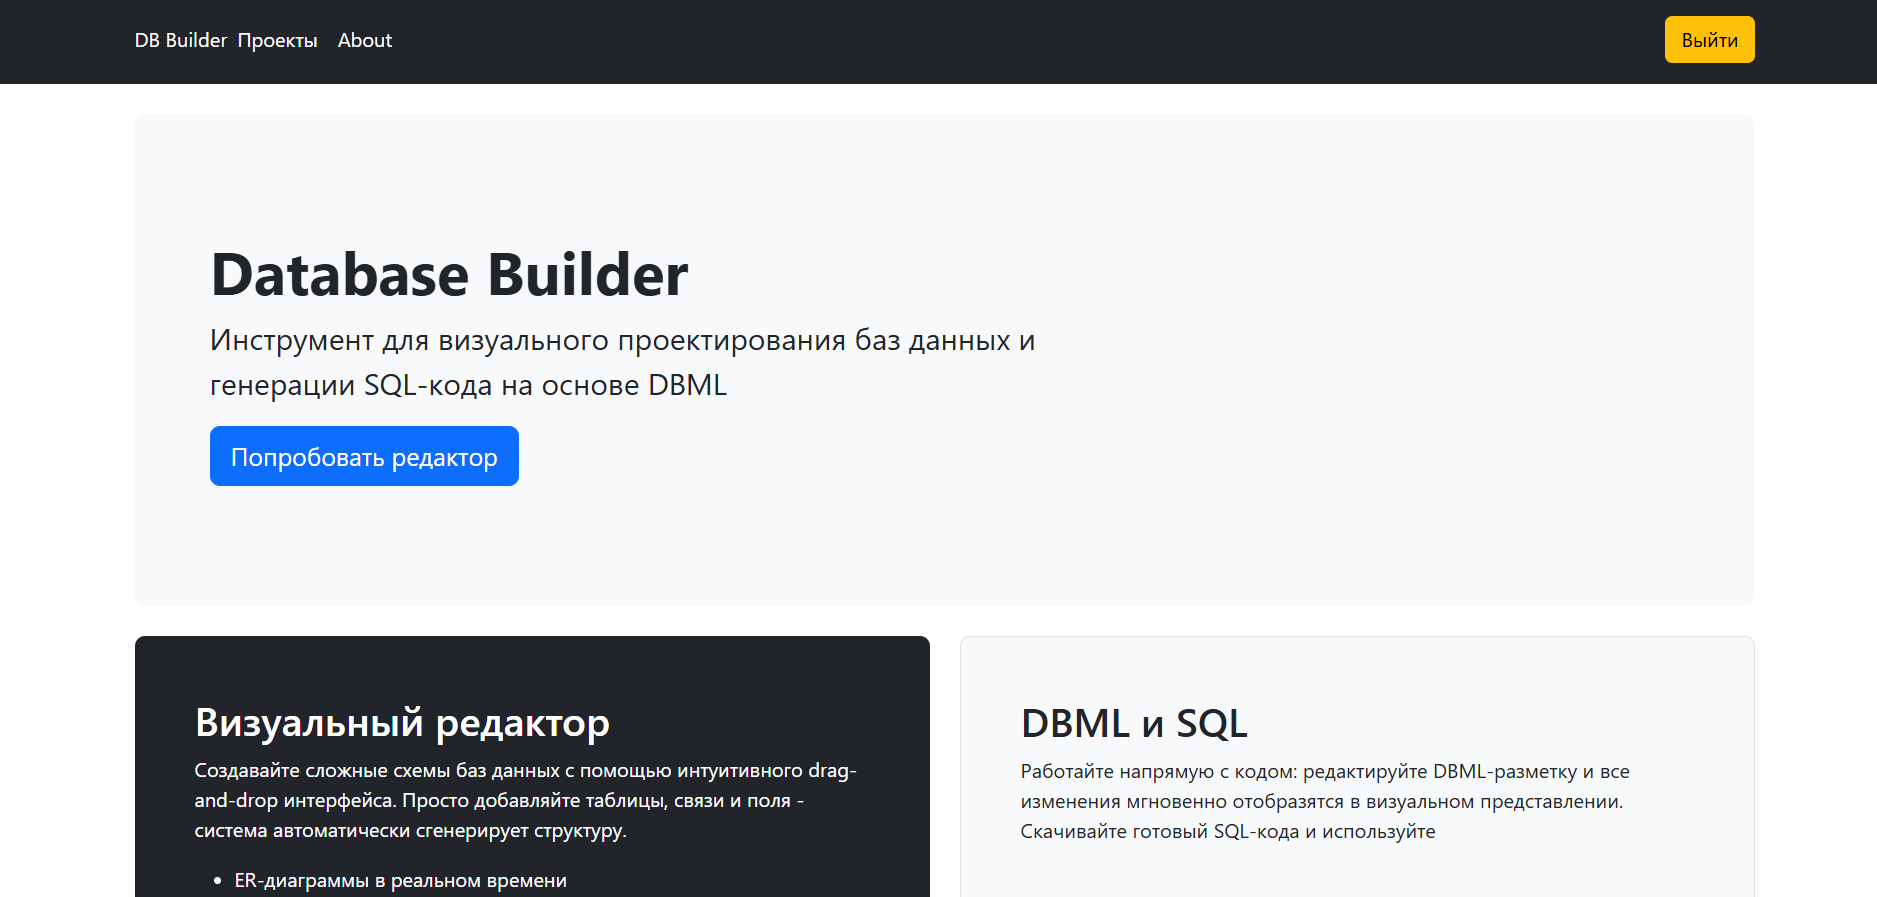
\includegraphics[height=0.45\textwidth]{img/home.png}
    \caption{Домашняя страница}
    \label{fig:analyze} % Метка для ссылок
\end{figure}

\textbf{\large 2.4.4 Страница проектов}
\addcontentsline{tocdepth}{subsubsection}{2.4.4 Страница проектов}

Эта страница содержит в себе все проекты, созданные пользователем (Рисунок 7). Интерфейс разделен на две части:

    - Левая панель - интерфейс для управления меню проектов. Содержит в себе логин пользователя и разделы "Мои проекты", "Общие диаграммы", "Избранное" и "Шаблоны".
    
    - Правая панель - список проектов, который может изменяться в зависимости от выбранного меню. Сверху находятся кнопка для создания нового проекта и кнопка сортировки.

У каждого проекта в левой верхней части есть три кнопки: для коллаборации, удаления и добавления проекта в избранное.

\renewcommand{\figurename}{Рисунок}
\begin{figure}[htbp]
    \centering % Центрируем изображение
    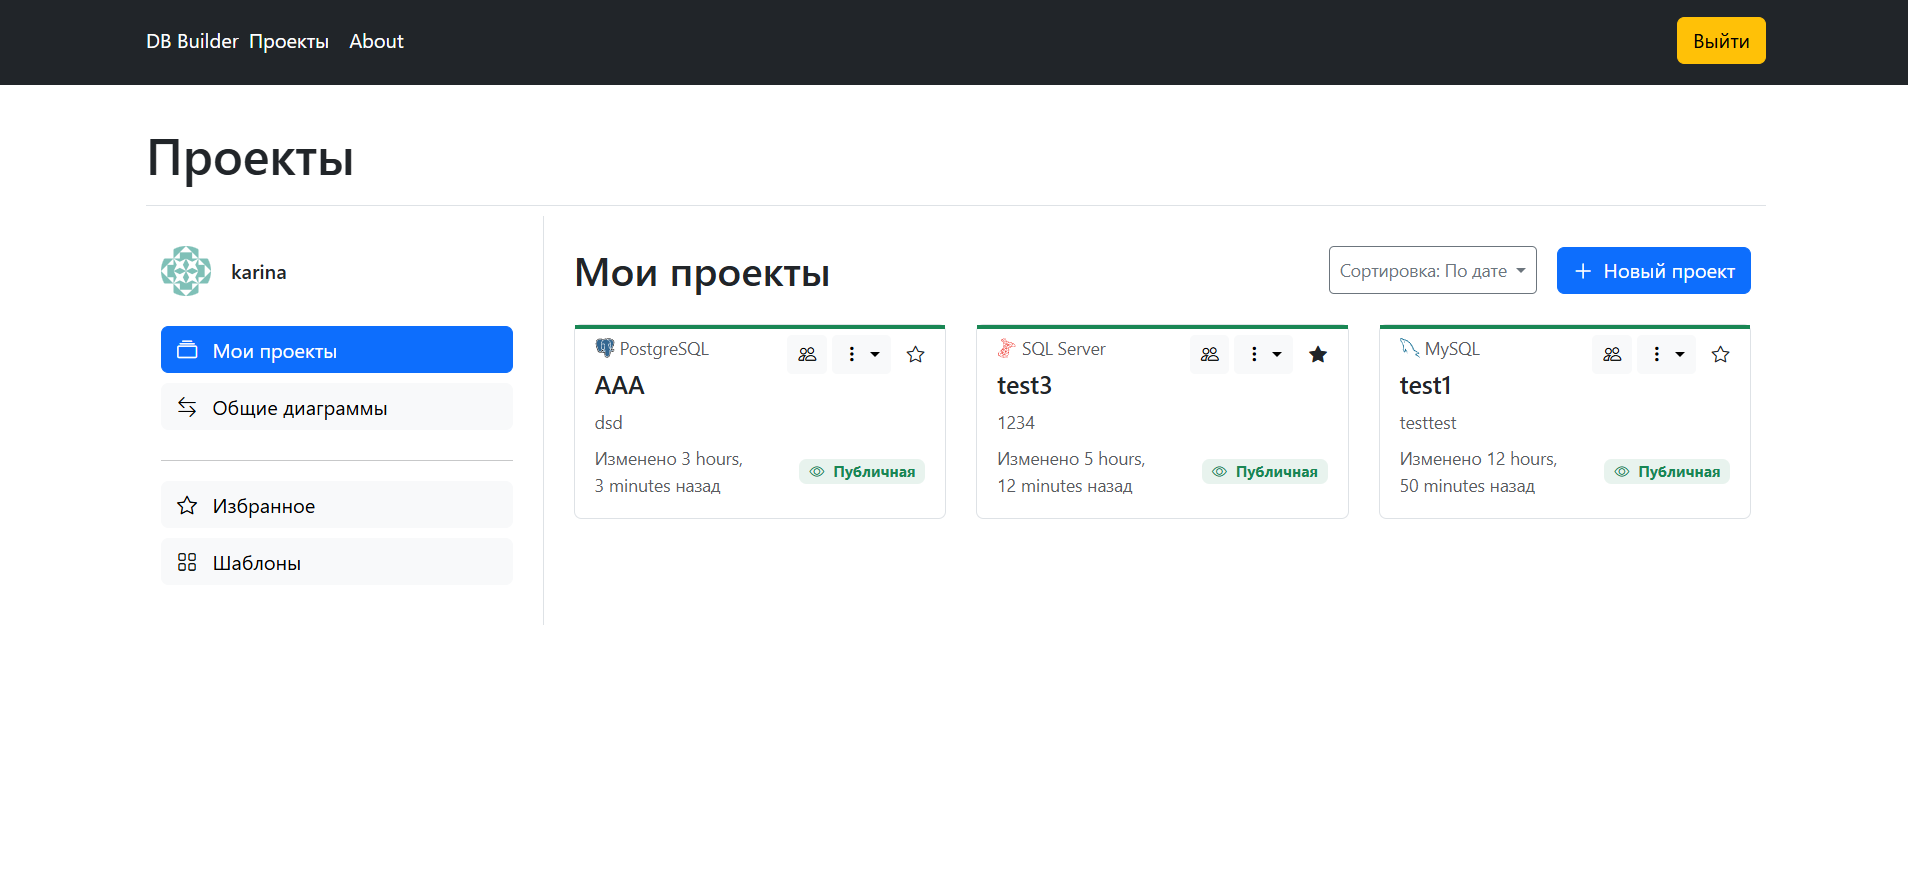
\includegraphics[height=0.45\textwidth]{img/projects.png}
    \caption{Страница проектов}
    \label{fig:analyze} % Метка для ссылок
\end{figure}

\newpage

\textbf{\large 2.4.5 Окно создания проекта}
\addcontentsline{tocdepth}{subsubsection}{2.4.5 Окно создания проекта}

Данное модальное окно (Рисунок 8) появляется на экране после нажатия пользователем кнопки "Новый проект". Интерфейс в нем разделен на две части:

    - Левая часть - информация для пользователя о создании проекта.
    
    - Правая часть - интерфейс для создания проекта. Содержит в себе поля ввода названия диаграммы, описания, радио-кнопки для выбора видимости диаграммы и кнопки для выбора типа базы данных.
    
Снизу находится кнопка "Создать диаграмму", после нажатия на которую, при условии ввода всех данных, пользователь возвращается на страницу проектов и в списке появляется новый проект.

\renewcommand{\figurename}{Рисунок}
\begin{figure}[htbp]
    \centering % Центрируем изображение
    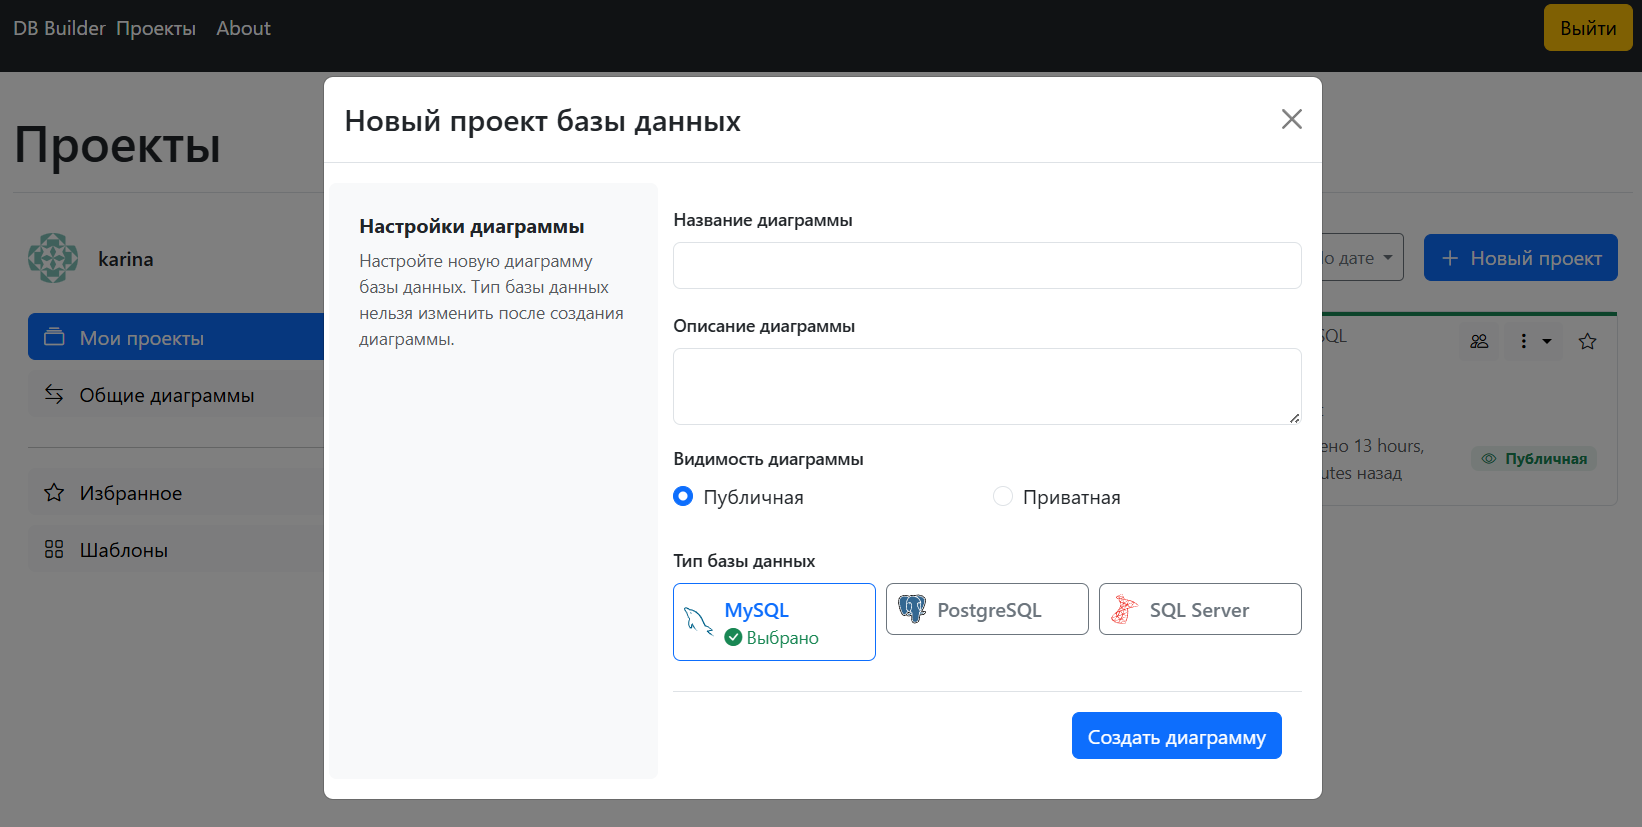
\includegraphics[height=0.45\textwidth]{img/new_project.png}
    \caption{Окно создания проекта}
    \label{fig:analyze} % Метка для ссылок
\end{figure}

\newpage

\textbf{\large 2.4.6 Окно управления доступом к проекту}
\addcontentsline{tocdepth}{subsubsection}{2.4.6 Окно управления доступом к проекту}

Данное модальное окно (Рисунок 9) появляется на экране после нажатия пользователем на иконку коллаборации в контекстном меню проекта. Интерфейс состоит из поля ввода электронного адреса пользователя, кнопки добавить, а также списка участников проекта. Возле логина каждого участника написана его роль в проекте. После нажатия на кнопку "Добавить" пользователь добавляется в проект и может вносить в него изменения. Возле логина участника проекта находится иконка крестика для удаления его из проекта.
    
\renewcommand{\figurename}{Рисунок}
\begin{figure}[htbp]
    \centering % Центрируем изображение
    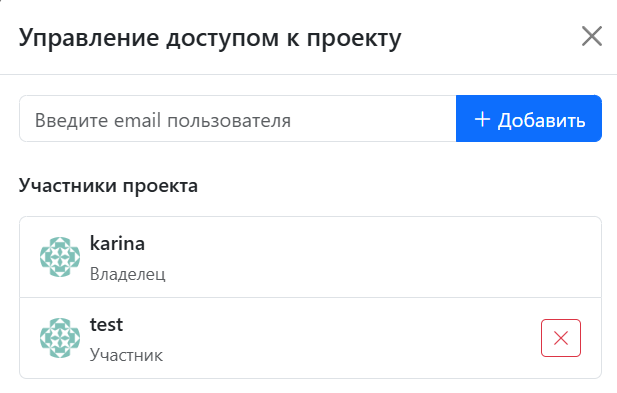
\includegraphics[height=0.45\textwidth]{img/permission.png}
    \caption{Окно управления доступом к проекту}
    \label{fig:analyze} % Метка для ссылок
\end{figure}

\newpage

\textbf{\large 2.4.7 Страница редактора}
\addcontentsline{tocdepth}{subsubsection}{2.4.7 Страница редактора}

Это основная страница для редактирования проекта (Рисунок 10). Сверху находится меню управления проектом, содержащее в себе кнопки для сохранения, экспорта SQL, смены темы, добавления и удаления узла. Кнопка "Сохранить" отвечает за ручное сохранение проекта, она необязательна, так в проекте реализовано автосохранение каждые 100мс. После нажатия на кнопку "Export SQL" происходит скачивание SQL представления проекта. При нажатии на кнопку "Добавить проект" создается новая таблица. При выделении курсором элемента и нажатии на кнопку "Удалить выбранное", выбранный элемент удаляется.

В левой панели располагается редактор DBML кода с синтаксической подсветкой, справа располагается панель с графический интерфейсом для создания диаграммы. У каждой таблицы в диаграмме есть кнопка "+" для добавления нового поля в таблицу. Рядом с каждым полем расположена кнопка крестика для удаления поля. При клике на тип поля появлется контекстное меню для замены значения. По обе стороны каждого поля находятся порты для связей между таблицами. Пользователь может создать связь между таблицами, протянув курсор от одного порта, к другому, либо прописать соответствующий DBML код. При клике правой кнопкой мыши на стрелку связи появляется контекстное меню для выбора типа связи: 1:1, 1:N или N:1. После смены выбора типа стрелки меняет внешний вид.
    
\renewcommand{\figurename}{Рисунок}
\begin{figure}[htbp]
    \centering % Центрируем изображение
    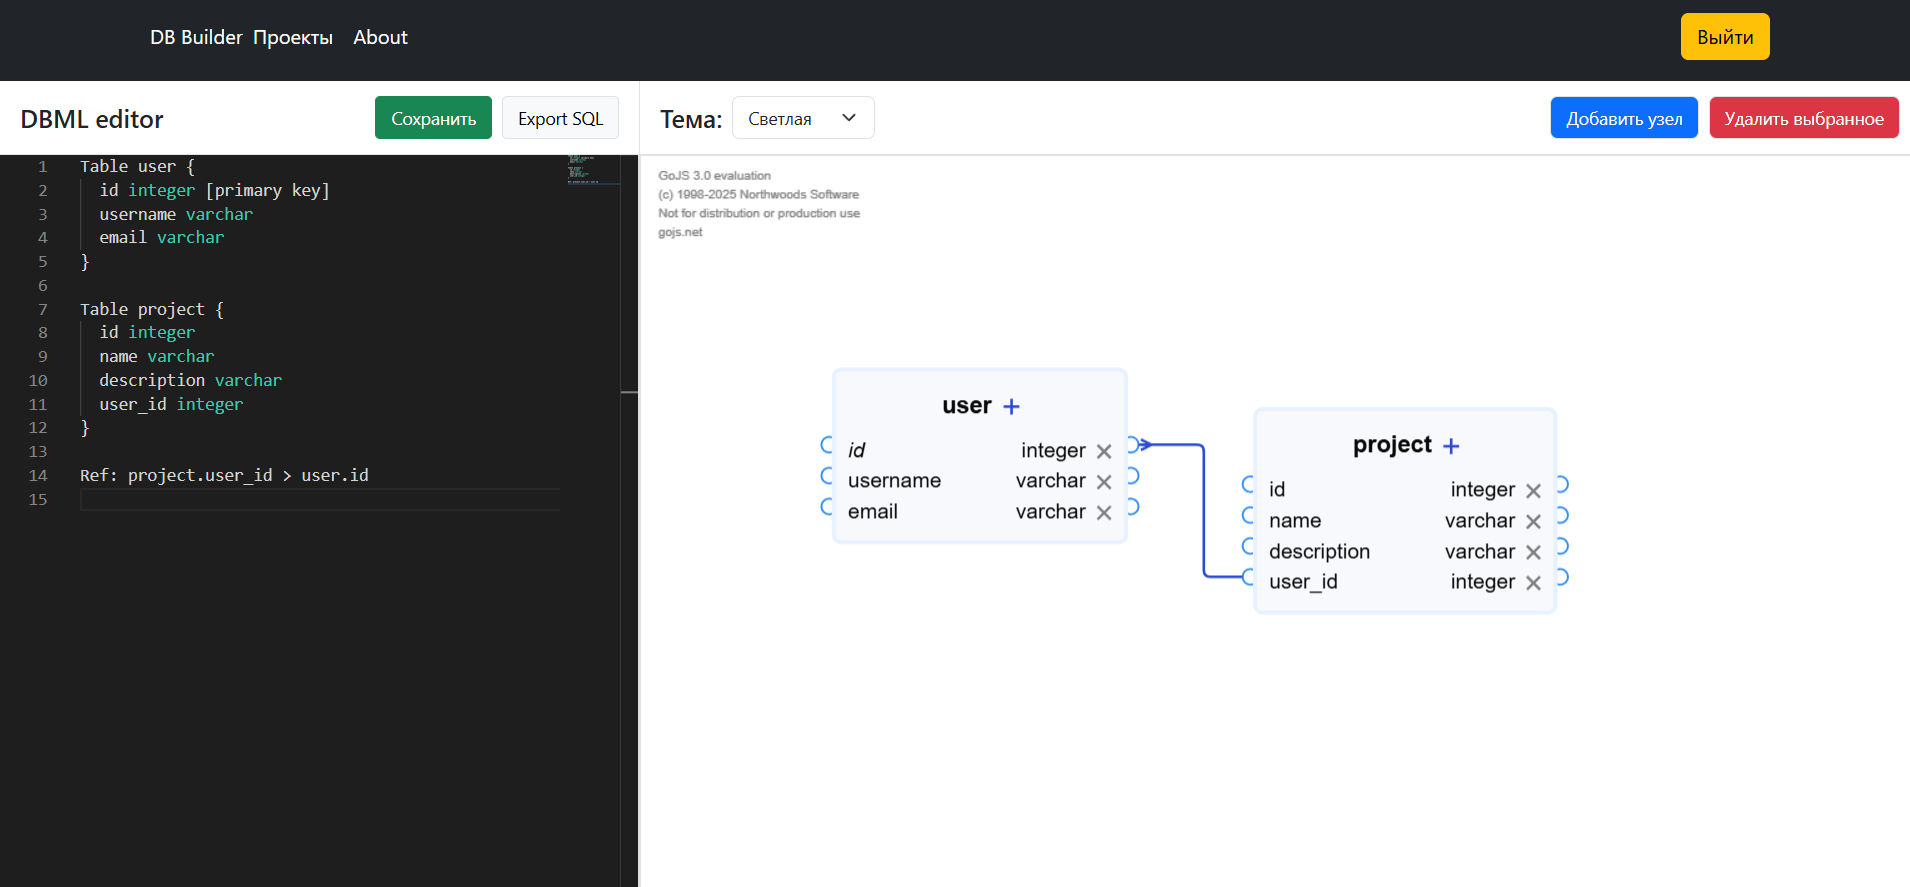
\includegraphics[height=0.45\textwidth]{img/builder.png}
    \caption{Страница редактора}
    \label{fig:analyze} % Метка для ссылок
\end{figure}

\textbf{\large 2.5 Техническая реализация}
\addcontentsline{toc}{subsection}{2.5 Техническая реализация}

Проект реализован на основе современного стека технологий, обеспечивающего кроссплатформенную работу и высокую производительность. В качестве клиентской части используется React-приложение с библиотекой GoJS для интерактивной визуализации диаграмм баз данных. Серверная часть построена на Django REST Framework, что обеспечивает надежное API для хранения и обработки данных.

Для работы с диаграммами баз данных применена библиотека GoJS, предоставляющая богатый набор инструментов для создания интерактивных схем. Визуальное представление таблиц и связей между ними реализовано через кастомизированные шаблоны узлов и соединений. Каждая таблица отображается как отдельный компонент с возможностью редактирования названий полей, типов данных и первичных ключей. Связи между таблицами поддерживают различные типы отношений с соответствующей визуализацией.

Редактор DBML-кода реализован на базе Monaco Editor — том же движке, что используется в Visual Studio Code. Это обеспечивает продвинутую подсветку синтаксиса, автодополнение и проверку ошибок в реальном времени. Для синхронизации между графическим представлением и текстовым редактором разработан специальный механизм преобразования.

Серверная часть реализована на Django с использованием следующих ключевых компонентов:

- модель Project для хранения DBML-схем и метаданных;

- API на базе Django REST Framework для безопасного доступа к данным;

- система аутентификации через JWT-токены;

- механизм контроля доступа к проектам.

Для хранения данных используется PostgreSQL с поддержкой JSON-полей, что позволяет эффективно сохранять структуру диаграмм и дополнительные метаданные.

Вся структура приложения разделена на отдельные модули: home, builder, users, DB\_Builder. Каждый модуль отвечает за отдельную функциональность. Это делает код легко поддерживаемым и
расширяемым. Базовый шаблон страниц вынесен в отдельный файл, что позволяет централизованно управлять внешним видом всех основных элементов интерфейса и не дублировать код.

Система обладает  двусторонней синхронизацией между графическим и текстовым представлением,
поддержка экспорта в SQL для разных СУБД, гибкой системой ролей и прав доступа

Такая архитектура обеспечивает высокую сопровождаемость кода и возможность дальнейшего расширения функциональности.

\

\textbf{\large 2.6 Выводы}
\addcontentsline{toc}{subsection}{2.6 Выводы}

В результате разработки было создано современное, удобное и
функциональное веб-приложение для визуального проектирования баз данных и генерации SQL-кода.

Программа реализует все заявленные возможности: авторизацию и
регистрацию пользователей, создание проектов, добавление других пользователей в проект, что реализует командную разработку, распределение ролей в проекте, добавление проекта в избранное, проектирование базы данных с помощью DBML кода, визуальное проектирование посредством графического интерфейса, синхронизация между графическим представлением проекта и DBML представлением, удобный редактор кода DBML с подстветкой синтаксиса.

Особое внимание уделялось безопасности хранения пользовательских
данных, производительности при работе с большим количеством таблиц и
удобству пользователя.

Проект демонстрирует эффективное сочетание современных веб-технологий для решения специализированной задачи проектирования баз данных. Реализованное решение может быть использовано как самостоятельный сервис или интегрировано в более крупные системы управления разработкой. Удобство использования, богатый функционал и надежная техническая реализация делают этот инструмент ценным для широкого круга пользователей — от студентов до профессиональных разработчиков баз данных.
